\chapter{Mathematical Model, Results and Analysis}\label{ch:results}

This chapter first states the system as a mathematical model (Section~\ref{sec:math}), exactly as the
code computes it, then the evaluation method (Section~\ref{sec:evalmethod}), the results with their
analysis (Sections~\ref{sec:baseline}--\ref{sec:speed}) and the testing (Section~\ref{sec:testing}).
All runs used the real models on the laptop GPU; each table names its source file in
\code{docs/results/} or \code{docs/testing/}.

\section{Mathematical model}\label{sec:math}

\subsection{Notation}
A photo is a map $I:\Omega\to[0,255]^3$ on the pixel grid $\Omega=\{1,\dots,H\}\times\{1,\dots,W\}$,
with channels $R,G,B$. For a set of pixels $A\subseteq\Omega$, $|A|$ is its number of pixels.
$B_r$ is the square structuring element of side $2r+1$; $\oplus$ and $\ominus$ are morphological
dilation and erosion.

\subsection{Vegetation mask}\label{sec:math-veg}
The excess-green index of Woebbecke et al.~\cite{woebbecke1995color} is computed per pixel,
\begin{equation}
  \mathrm{ExG}(p) = 2G(p) - R(p) - B(p), \qquad p\in\Omega .
\end{equation}
Its threshold $\tau^\ast$ is chosen per photo by Otsu's method: for a candidate threshold $t$ let
$\omega_0(t),\omega_1(t)$ be the fractions of pixels below and above $t$ and $\mu_0(t),\mu_1(t)$ their
mean ExG. The threshold maximises the between-class variance,
\begin{equation}
  \tau^\ast = \arg\max_t\; \sigma_b^2(t) = \arg\max_t\; \omega_0(t)\,\omega_1(t)\,\bigl(\mu_0(t)-\mu_1(t)\bigr)^2 ,
\end{equation}
and the vegetation mask is $V=\{p\in\Omega : \mathrm{ExG}(p) > \tau^\ast\}$.

\subsection{Plant patches}
Leaves of one plant are often separated by a few pixels, so gaps are closed before connected
components are taken:
\begin{equation}
  V' = (V \oplus B_r)\ominus B_r,\qquad r=\max\bigl(1,\operatorname{round}(0.01\max(H,W))\bigr).
\end{equation}
The plant patches $P_1,\dots,P_n$ are the 8-connected components of $V'$, each restricted to real
vegetation ($P_k\leftarrow P_k\cap V$); patches with $|P_k|<12$ pixels are ignored.

\subsection{Crop reference and planting rows}
Let $M_1,\dots,M_m$ be the SAM~2 masks whose detector label names the crop (and no weed), with masks
covering more than half of the photo removed. Their union is $C=\bigcup_j M_j$, the crop overlap of a
patch is $o(P)=|P\cap C|/|P|$, and the typical crop size is the median
\begin{equation}
  \tilde m = \operatorname{median}_j\, |M_j\cap V| .
\end{equation}
For the rows, the vegetation is summed along each image axis, e.g.\ $h(y)=\sum_x V(x,y)$, and smoothed
with a 15-pixel moving average to $\tilde h$. The axis with the larger peakiness
$\pi=\max\tilde h/\overline{\tilde h}$ is the row direction, and the photo has \emph{clear rows} iff
$\pi\ge 2$. A patch with centroid coordinate $c(P)$ across the rows lies \emph{on the row} iff
$\tilde h\bigl(c(P)\bigr)\ge 0.5\max\tilde h$.

\subsection{Plant classifier}
The four rules of Section~\ref{sec:rules} form a piecewise function, evaluated top to bottom:
\begin{equation}\label{eq:rules}
f(P)=\begin{cases}
\text{crop}   & \text{if } o(P)\ge 0.3,\\
\text{crop}   & \text{else if rows} \wedge \text{on-row}(P),\\
\text{weed}   & \text{else if } C\neq\emptyset \wedge |P| < 0.25\,\tilde m,\\
\text{unsure} & \text{else if } C\neq\emptyset,\\
\text{weed}   & \text{else if rows} \wedge \neg\,\text{on-row}(P),\\
\text{unsure} & \text{otherwise.}
\end{cases}
\end{equation}
Note the fifth line: the off-row rule is reached only when the photo has \emph{no} crop mask
($C=\emptyset$). That is exactly the situation of finding F1 (Section~\ref{sec:f1}).

\subsection{Safety gate}\label{sec:math-gate}
Each detection $i$ has a box, a label $\ell_i$, a confidence $s_i$, a SAM~2 mask $M_i$ and a predicted
mask quality $q_i$. With $\mathcal W(\ell)$ true when the label names a weed and $\mathcal C(\ell)$ true
when it names the crop, the gate approves a detector mask iff
\begin{equation}
  g_i = \mathcal W(\ell_i)\wedge\neg\,\mathcal C(\ell_i)\wedge s_i\ge\theta_s\wedge q_i\ge\theta_q\wedge
        \frac{|M_i|}{|\Omega|}\le 0.5,\qquad \theta_s=0.70,\ \theta_q=0.85 .
\end{equation}
The plant-rule weed set is $W_r=\bigcup_{f(P)=\text{weed}}P\setminus(C\cup C_r)$, where $C_r$ is the
union of patches classified as crop, so the nozzle never fires over a crop pixel. The spray map and
the infestation are
\begin{equation}
  S_0=\bigcup_{i:\,g_i}M_i\;\cup\;W_r,\qquad \iota=\frac{|S_0|}{|\Omega|},\qquad
  S=\begin{cases}S_0 & \iota\le 0.85\\ \emptyset & \iota>0.85\end{cases}
\end{equation}
In the application, the nozzle footprint is $S\oplus B_b$ for a buffer of $b$ pixels (default 10).

\subsection{Escalation agent}\label{sec:math-agent}
Source $k$ answers ``weed'' or ``crop'' with stated confidence $c_k$; its accuracy $a_k$ was measured
on 20 labelled patches (row rule 0.65, Clef Flash 0.70, Qwen VLM 0.80). The probability that the
answer is right, and from it the probability of ``weed'', are
\begin{equation}
  r_k = a_k c_k + (1-a_k)(1-c_k),\qquad
  p_k=\begin{cases} r_k & \text{answer ``weed''}\\ 1-r_k & \text{answer ``crop''}\end{cases},
\end{equation}
clipped to $[0.02,0.98]$. Assuming the sources err independently, the odds multiply from even odds
(a naive Bayes combination):
\begin{equation}
  O=\prod_k\frac{p_k}{1-p_k},\qquad P(\text{weed})=\frac{O}{1+O},\qquad
  \text{verdict}=\begin{cases}\text{weed} & P\ge 0.85\\ \text{crop} & P\le 0.15\\ \text{unsure} & \text{otherwise.}\end{cases}
\end{equation}
Since $r_k\le a_k\le 0.80<0.85$, one source alone can never reach a verdict. Two agreeing sources can:
for Clef ($a=0.70$) and Qwen ($a=0.80$) both certain, $O=\frac{0.7}{0.3}\cdot\frac{0.8}{0.2}=9.33$ and
$P=0.90$. Two sources that disagree with equal strength cancel to $O=1$, $P=0.5$, ``unsure''.

\subsection{Evaluation metrics}\label{sec:math-metrics}
Labels are boxes, so ground truth is vegetation inside boxes. With crop boxes $\{b^c_j\}$ and weed
boxes $\{b^w_j\}$,
\begin{equation}
  G_c = V\cap\bigcup_j b^c_j,\qquad G_w=\Bigl(V\cap\bigcup_j b^w_j\Bigr)\setminus G_c .
\end{equation}
Summed over all photos of a set (pooled, not averaged per photo):
\begin{align}
  \text{Crop sprayed (\%)} &= 100\,\frac{\sum|S\cap G_c|}{\sum|G_c|} &&\text{(damage, lower is better)}\\
  \text{Weed recall (\%)}  &= 100\,\frac{\sum|S\cap G_w|}{\sum|G_w|} &&\text{(higher is better)}\\
  \text{Herbicide saved (\%)} &= 100\Bigl(1-\frac{\sum|S|}{\sum|\Omega|}\Bigr) &&\text{(against blanket spraying)}
\end{align}
At plant level, a crop plant $j$ is \emph{touched} if $|S\cap V\cap b^c_j|>0$, and a weed is \emph{hit}
if at least half its vegetation pixels are sprayed. For mask quality, the usual
$\mathrm{IoU}(A,B)=|A\cap B|/|A\cup B|$ and $\mathrm{Dice}(A,B)=2|A\cap B|/(|A|+|B|)$ are implemented.
The metric code has unit tests built from three hand-computed $5\times5$ grids, for example crop
$2/6=33.3\%$, weed recall $3/4=75\%$ and saving 80\%.

\subsection{Complexity}
Vegetation, closing, connected components and rows are each $O(HW)$; the rules add $O(n)$ for $n$
patches, so System~1's own logic is linear in the image size. Photos larger than 1024~px on the long
side are subsampled for the rules and the result is upsampled back. Run time is dominated by the two
neural networks (Section~\ref{sec:speed}).

\section{Evaluation method}\label{sec:evalmethod}

\subsection{A fabricated evaluation set, found and replaced}
The first evaluation set (\code{eval\_manifest\_v1}, 20 images) looked real but was a template: every
sugar beet image carried the same two crop and six weed boxes, and every cotton image a cotton box,
although the official cotton dataset labels no cotton at all. Only one or two of eight boxes per beet
image matched the official labels, and none per cotton image (Figure~\ref{fig:audit}). A metric
reported on it earlier was meaningless and was withdrawn. It was replaced by \code{eval\_manifest\_v2},
built by a script that copies boxes from the official XML files; rebuilding it from a fresh download
gives an identical manifest.

\begin{figure}[H]
\centering
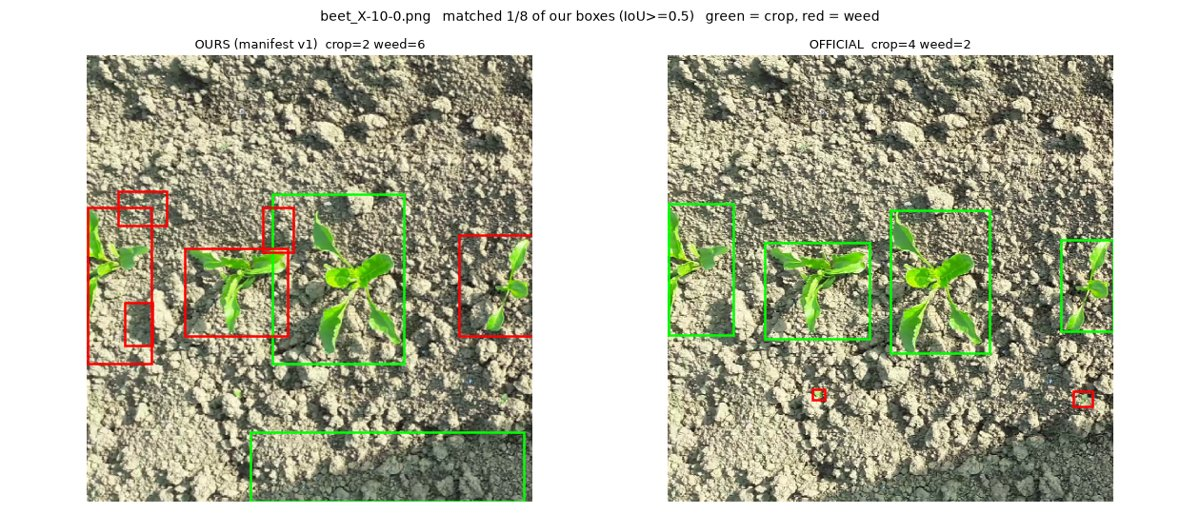
\includegraphics[width=0.49\textwidth]{audit_beet_X-10-0}\hfill
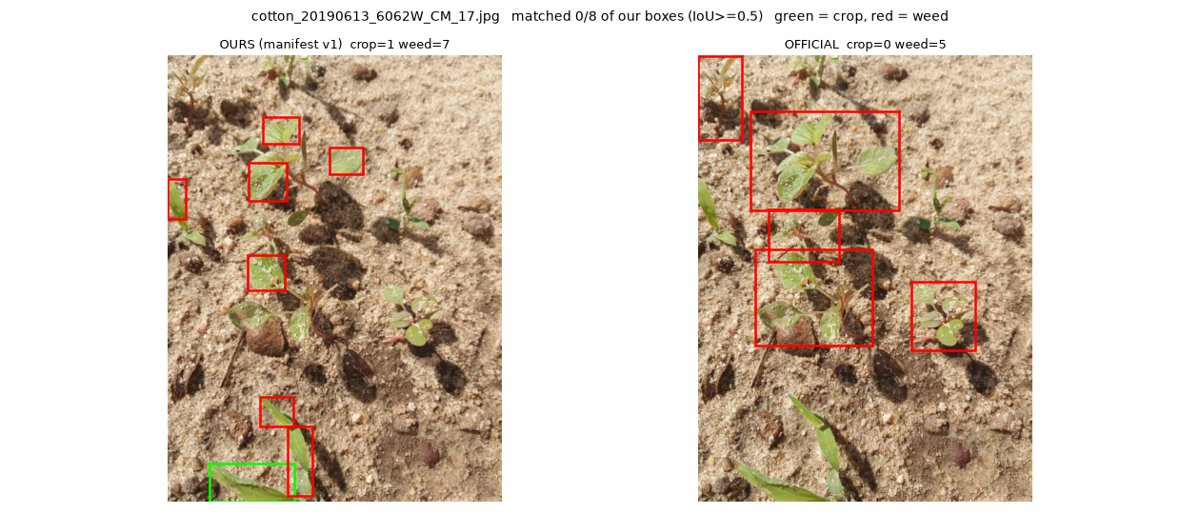
\includegraphics[width=0.49\textwidth]{audit_cotton_CM_17}
\caption{Label audit. Left: beet X-10-0, old labels put a ``crop'' box on bare soil and ``weed'' boxes on
beets. Right: cotton CM\_17, no old box matches the official weed boxes.}\label{fig:audit}
\end{figure}

\subsection{Development and held-out sets}
\begin{table}[H]
\centering
\caption{Evaluation sets. All labels are copied unchanged from the official files.}\label{tab:sets}
\begin{small}
\begin{tabularx}{\textwidth}{@{}L{4.3cm}L{2.1cm}L{3.1cm}Y@{}}
\toprule
\textbf{Set} & \textbf{Photos} & \textbf{Labels} & \textbf{Use}\\
\midrule
\code{eval\_manifest\_v2} (development) & 30 beet + 8 cotton & 93 beets, 282 weeds; 19 cotton weeds & Every design decision and every variant.\\
\code{eval\_manifest\_v2\_holdout} & 90 beet & 363 beets, 215 weeds & Run \textbf{once}, on 18 October, after the rules were frozen.\\
\bottomrule
\end{tabularx}
\end{small}
\end{table}
The held-out set is every sugar beet photo not in the development set. A repeat on 23 October
reproduced every number exactly, and a run of the first ten photos twice gave zero differences: the
pipeline is deterministic.

\subsection{Settings compared}
\begin{table}[H]
\centering
\caption{Settings compared. Prompt \code{weed . <crop> plant .}, detector box threshold 0.35, buffer 10~px.}\label{tab:settings}
\begin{small}
\begin{tabularx}{\textwidth}{@{}lY@{}}
\toprule
\textbf{Setting} & \textbf{Meaning}\\
\midrule
\code{every\_mask} & Spray every SAM~2 mask, whatever its label: the upper bound on recall and on damage.\\
\code{gate\_0.35}, \code{0.50}, \code{0.70} & Grounded SAM label policy with confidence floor $\theta_s$ = 0.35, 0.50 or 0.70 (0.70 is deployed).\\
\code{+exclusion} & Also subtract crop-labelled masks from weed masks before spraying.\\
\code{plant\_rules} & The deployed product: plant rules v3 plus the gate.\\
agent & Deployed gate plus the escalation agent reviewing up to three withheld plants per photo.\\
\bottomrule
\end{tabularx}
\end{small}
\end{table}

\section{Baseline: Grounded SAM label policy (RQ1)}\label{sec:baseline}
\begin{table}[H]
\centering
\caption{Sugar beet development set (30 photos).}\label{tab:baseline}
\begin{small}
\begin{tabularx}{\textwidth}{@{}L{4.3cm}RRRRR@{}}
\toprule
\textbf{Setting} & \textbf{Crop sprayed \%} & \textbf{Weed recall \%} & \textbf{Saved \%} & \textbf{Beets touched} & \textbf{Weeds hit}\\
\midrule
every\_mask & 93.9 & 97.6 & 39.3 & 87/93 & 265/282\\
gate\_0.35 & 70.8 & 9.0 & 93.0 & 45/93 & 7/282\\
gate\_0.50 & 20.5 & 6.8 & 98.0 & 8/93 & 1/282\\
gate\_0.70 (deployed) & 0.0 & 0.0 & 100.0 & 0/93 & 0/282\\
\bottomrule
\end{tabularx}
\end{small}
\src{docs/results/baseline_v2_20261018.md}
\end{table}

\textbf{Analysis.} SAM~2 outlines plants well: spraying every mask reaches 97.6\% weed recall. The
problem is the labels. At a confidence floor of 0.35 the label policy sprays 70.8\% of crop pixels
while hitting only 9\% of weed pixels: the detector calls crop plants ``weed'' more often than it
finds the real weeds. Real Grounding DINO scores on these photos never exceeded 0.68, so the deployed
gate at 0.70 sprays nothing at all: perfectly safe and perfectly useless. On cotton, spraying every
mask hits 75.8\% of weed pixels, but every gated setting hits 0\%. \textbf{Answer to RQ1:} text prompts
alone do not separate crop from weed on these photos; lowering the gate buys recall only by spraying
the crop. This agrees with Chong et al.~\cite{chong2025zeroshot}.

\section{Cheap additions: crop exclusion, thresholds, tiling (RQ3)}\label{sec:cheap}
\begin{table}[H]
\centering
\caption{Crop exclusion and detector variants, sugar beet development set.}\label{tab:cheap}
\begin{small}
\begin{tabularx}{\textwidth}{@{}L{5.0cm}RRRR@{}}
\toprule
\textbf{Setting} & \textbf{Crop sprayed \%} & \textbf{Weed recall \%} & \textbf{Beets touched} & \textbf{s / photo}\\
\midrule
gate\_0.35 & 70.8 & 9.0 & 45/93 & 0.58\\
gate\_0.35 + exclusion & 50.1 & 9.0 & 38/93 & 0.58\\
gate\_0.50 & 20.5 & 6.8 & 8/93 & 0.58\\
gate\_0.50 + exclusion & \textbf{5.3} & 6.8 & 2/93 & 0.58\\
box threshold 0.20, gate\_0.50 + exclusion & 0.0 & 0.4 & 0/93 & 1.03\\
$2\times2$ tiles, gate\_0.35 & 74.6 & 10.1 & 49/93 & 3.76\\
\bottomrule
\end{tabularx}
\end{small}
\src{docs/results/exclusion_v2_20261018.md, detector_variants_20261018.md}
\end{table}

\textbf{Analysis.} Subtracting crop masks from weed masks cut crop pixels sprayed from 20.5\% to 5.3\%
at a 0.50 floor with no loss of recall. Running the detector on $2\times2$ tiles, or with a lower box
threshold, finds more plants but labels them no better, and slows the pipeline up to 13 times. The
bottleneck is classification, not detection. Plant-sized SAM~2 masks from detector boxes covered only
about 9\% of the beet weed pixels; the 97.6\% of \code{every\_mask} comes largely from masks covering the
whole photo.

\section{Plant rules on the development set}
\begin{table}[H]
\centering
\caption{Plant rules v3, sugar beet development set.}\label{tab:rulesdev}
\begin{small}
\begin{tabularx}{\textwidth}{@{}L{4.3cm}RRRRR@{}}
\toprule
\textbf{Setting} & \textbf{Crop sprayed \%} & \textbf{Weed recall \%} & \textbf{Saved \%} & \textbf{Beets touched} & \textbf{Weeds hit}\\
\midrule
every\_plant\_mask & 84.7 & 9.1 & 91.6 & 53/93 & 8/282\\
gate\_0.50 + exclusion & 5.3 & 6.8 & 99.3 & 2/93 & 1/282\\
\textbf{plant\_rules (v3)} & \textbf{4.6} & \textbf{71.5} & 90.5 & 21/93 & 219/282\\
\bottomrule
\end{tabularx}
\end{small}
\src{docs/results/plant_rules_v3_20261018.md, pipeline_plant_rules_dev_20261020.md}
\end{table}

\section{Held-out result (the headline)}\label{sec:holdout}
\begin{table}[H]
\centering
\caption{Held-out sugar beet set (90 photos, evaluated once).}\label{tab:holdout}
\begin{small}
\begin{tabularx}{\textwidth}{@{}L{4.3cm}RRRRR@{}}
\toprule
\textbf{Setting} & \textbf{Crop sprayed \%} & \textbf{Weed recall \%} & \textbf{Saved \%} & \textbf{Beets touched} & \textbf{Weeds hit}\\
\midrule
every\_mask & 94.4 & 93.2 & 60.2 & 334/363 & 204/215\\
Grounded SAM, gate\_0.35 & 65.5 & 1.8 & 85.0 & 242/363 & 3/215\\
Grounded SAM, gate\_0.50 & 22.5 & 0.0 & 95.5 & 49/363 & 0/215\\
Grounded SAM, gate\_0.70 (deployed) & 0.0 & 0.0 & 100.0 & 0/363 & 0/215\\
gate\_0.50 + exclusion & 5.5 & 0.0 & 98.8 & 24/363 & 0/215\\
\textbf{plant\_rules (v3), the product} & \textbf{8.8} & \textbf{77.9} & 95.0 & 104/363 & 177/215\\
\bottomrule
\end{tabularx}
\end{small}
\src{docs/results/holdout_plant_rules_v3_20261018.md}
\end{table}

\begin{figure}[H]
\centering
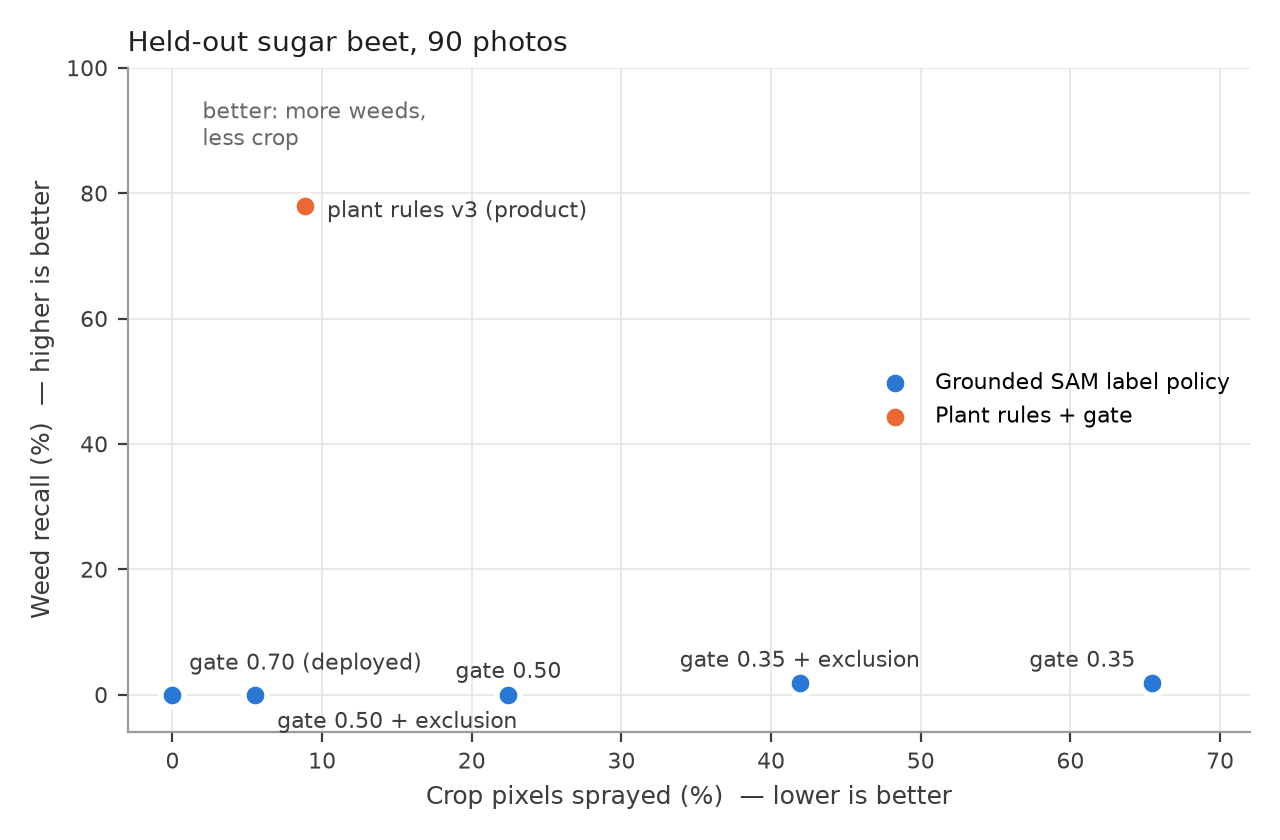
\includegraphics[width=0.78\textwidth]{tradeoff_holdout}
\caption{Crop pixels sprayed against weed recall on the held-out set. Every Grounded SAM setting lies on
the left edge (almost no weeds hit); the plant rules move the operating point to 77.9\% recall at 8.8\%
crop sprayed.}\label{fig:tradeoff}
\end{figure}

\textbf{Analysis.} On photos it had never seen, the product hits 77.9\% of weed pixels (177 of 215
weeds) and sprays 8.8\% of crop pixels, against 1.8\% and 65.5\% for the best-recall Grounded SAM
setting, while saving 95\% of the herbicide of blanket spraying. Held-out recall is higher than on the
development set (71.5\%), so there is no sign of overfitting the rules to the development photos. The
cost is real: 104 of 363 beets have at least one sprayed pixel, mostly small specks at a plant's edge,
but some whole plants (Section~\ref{sec:f1}). On the eight cotton photos the rules reach only 10.4\%
weed recall: rule~3 assumes weeds are smaller than the crop, true for young sugar beet and false for
cotton close-ups where one large weed fills the photo.

\textbf{Is a held-out set of 90 photos enough?} No model was trained or fine-tuned in this project, so
the 120 sugar beet photos are evaluation data only, and they are the complete public
dataset~\cite{data_sugarbeets}, not a sample from it. The held-out part contains 363 crop plants and
215 weeds. At plant level, the 95\% Wilson confidence interval for the share of weeds hit is
76.7--86.8\% (177/215) for the plant rules against 0.5--4.0\% (3/215) for the best-recall Grounded
SAM setting; for crop plants touched it is 24.2--33.5\% (104/363) against 61.7--71.3\% (242/363).
The intervals are far apart, so the size of the test set limits how precisely the numbers are known,
not the conclusion. What the data cannot show is generality beyond young sugar beet in one dataset,
which is why our claims are stated for that crop only.

\section{Escalation agent (RQ2)}\label{sec:agent-results}
\begin{table}[H]
\centering
\caption{Verdicts of the escalation agent on 69 withheld plants, development set, deployed gate.}\label{tab:agent}
\begin{small}
\begin{tabularx}{0.8\textwidth}{@{}YRRR@{}}
\toprule
\textbf{Plant really was} & \textbf{Agent: weed} & \textbf{Agent: crop} & \textbf{Agent: unsure}\\
\midrule
crop (44) & 0 & 13 & 31\\
weed (25) & 0 & 1 & 24\\
\bottomrule
\end{tabularx}
\end{small}
\src{docs/results/agent_v2_20261018.md}
\end{table}

\textbf{Analysis.} The agent reviewed up to three withheld plants per photo (69 in total, about 40
minutes; 14 of 69 Groq calls were lost to the free tier's per-minute limit and counted as ``no
answer''). It never approved spraying a crop plant, and 13 of its 14 ``crop'' verdicts were right. But
it called none of the 25 real weeds a weed, so the spray map was identical with and without it.
\textbf{Answer to RQ2:} escalation to vision-language models, combined conservatively, is safe and
precise but not effective for the crop-versus-weed decision on this data. The rules reach 77.9\%
recall with no model calls at all; the agent stays in the product, off by default, as a reviewer that
explains withheld plants.

\section{Vision-language models as a second opinion}
\begin{table}[H]
\centering
\caption{Crop-or-weed answers on 20 labelled plant patches (10 beet crop, 6 beet weed, 4 cotton weed).}\label{tab:vlm}
\begin{small}
\begin{tabularx}{\textwidth}{@{}YRRR@{}}
\toprule
\textbf{Source} & \textbf{Correct} & \textbf{Crop called crop} & \textbf{Weed called weed}\\
\midrule
Qwen~3.8 27B on Groq, told the crop & 16/20 & 9/10 & 7/10\\
Qwen~3.8 27B on Cloudflare, same prompt & 12/20 & 5/10 & 7/10\\
Clef Flash (Cloudflare) & 14/20 & 8/10 & 6/10\\
Row rule, no model & 13/20 & 7/10 & 6/10\\
\bottomrule
\end{tabularx}
\end{small}
\src{docs/results/t2_2_crop_or_weed_groq_20261017.json, qwen_provider_check_20261030.md}
\end{table}
Twenty patches is a small sample, but two lessons hold. First, the same model name gave 16 of 20 from
one provider and 12 of 20 from another (finding F25), so the agent's accuracy weights $a_k$ are tied to
the provider they were measured on. Second, in the sugar beet data the weeds are tiny (median 16~px
across) and the crops large (median 68~px), so size alone separates many cases; this is why rule~3
works on beet and not on cotton.

\section{Main limitation: rule 4 and whole beets (F1)}\label{sec:f1}
Rule~4 calls any off-row patch a weed whatever its size, and by Equation~\eqref{eq:rules} it applies
exactly when the detector found no crop. When photo X-10-0 was rotated by 90\textdegree, the detector
returned no crop box and the largest beet (4,410~px) was sprayed completely (Figure~\ref{fig:f1}). A
size limit on rule~4 was measured on the development set only:
\begin{table}[H]
\centering
\caption{The size limit trades recall for crop safety (development set).}\label{tab:f1}
\begin{small}
\begin{tabularx}{\textwidth}{@{}YRRR@{}}
\toprule
\textbf{Rule 4 applies up to \ldots{} $\times$ the median on-row plant} & \textbf{Crop sprayed \%} & \textbf{Weed recall \%} & \textbf{Beets mostly sprayed}\\
\midrule
0.25 & 0.25 & 12.9 & 0\\
1.0 & 0.98 & 31.3 & 3\\
1.5 & 1.20 & 39.1 & 4\\
no limit (v3, frozen) & 4.55 & 71.5 & 11\\
\bottomrule
\end{tabularx}
\end{small}
\src{scripts/experiment_f1_row_rule.py; docs/testing/Verification_Report_20261023.md}
\end{table}
Rule~4 gives most of the recall and most of the damage. We kept v3 frozen, because no unused held-out
set is left to test a changed rule fairly, and report the trade-off; a ``safe mode'' with the size limit
is future scope.

\begin{figure}[H]
\centering
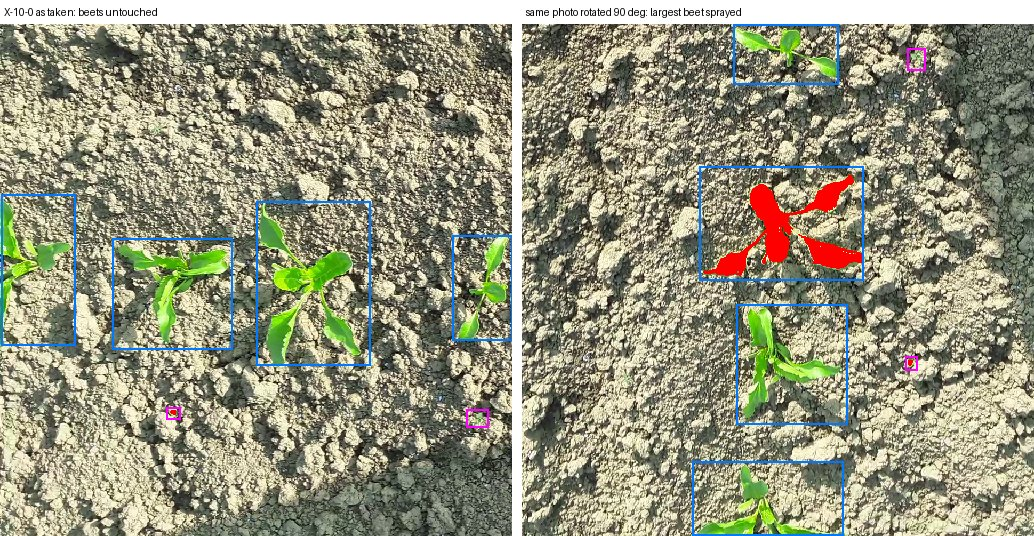
\includegraphics[width=0.85\textwidth]{verify_rotation_X-10-0}
\caption{Finding F1. Photo X-10-0 rotated by 90\textdegree: the detector returns no crop box, so rule~4
marks the largest beet as an off-row weed and it is sprayed completely.}\label{fig:f1}
\end{figure}

\section{ICAR herbicide table check}\label{sec:icar}
Every herbicide row and dose ceiling in the code was compared with the rendered pages of the
bulletin~\cite{choudhury2016icar} (\code{docs/results/icar\_table\_check\_20261020.md}). Eight cotton rows
were correct; two had a missing value stored as 0 instead of ``not stated''. The rice row for
pyrazosulfuron-ethyl was dangerous: 20~g a.i./ha with a 75-day waiting period, against the bulletin's
10--15~g and 95 days, an overdose with a shorter waiting period. It and six other values were
corrected, and all nine banned, withdrawn and refused herbicides matched. Regression tests fail on the
old values. In a manual test on cotton photo CM\_17, System~2 named the weed \emph{Amaranthus} (correct
genus) and matched a real ICAR cotton row: pyrithiobac-sodium 10\% EC, 75~g a.i./ha, waiting period 160
days, bulletin page 35.

\section{Speed}\label{sec:speed}
The pipeline takes 0.56--0.64~s per photo on the RTX~5050 after the first photo (detection 0.21~s,
segmentation 0.27--0.37~s), inside NFR3. Loading both models takes 4--14~s and happens once per
application process. A real run in the application, including the cloud diagnosis, takes about 15~s,
or about 40~s with the escalation agent. On the 4~GB RTX~3050 of the second test cycle the first real
run took 3.6~s.

\section{Testing}\label{sec:testing}
\begin{table}[H]
\centering
\caption{Testing summary.}\label{tab:testing}
\begin{small}
\begin{tabularx}{\textwidth}{@{}L{3.2cm}YL{3.0cm}@{}}
\toprule
\textbf{Level} & \textbf{What} & \textbf{Result}\\
\midrule
Unit & 235 tests: gate rules, plant rules, metrics (hand-computed grids), ICAR rows vs bulletin, GeoJSON geometry, providers, farmer summary, model cache, verdict view. & all pass\\
End to end & 35 tests through the workflow and the app in mock mode. & all pass\\
Static & ruff, ruff format, mypy on \code{src/}. & clean\\
CI & GitHub Actions on every push, Python 3.11 and 3.13. & green\\
System cycle 0 (16 Oct) & 16 app test cases on a fresh Windows install (Amit Ingle). & 7 pass, 9 fail $\rightarrow$ 8 issues, all fixed\\
Headless regression & The app driven by Streamlit AppTest in mock and real mode. & all pass\\
Verification run (23 Oct) & Fresh clone, data rebuild, held-out reproduction, determinism, 12 edge-case images, no-network run. & reproduces exactly; 13 findings\\
Manual cycle (30 Oct) & MT-01 \ldots{} MT-10 on six test photos, real mode. & core cases pass; 16 findings\\
System cycle 2 (7--8 Nov) & Final build on Windows~11, Python 3.13, RTX~3050 (4~GB), real mode: install, automated checks, regression of F24--F29, manual and exploratory cases (Amit Ingle). & 24/24 executed cases pass; 1 finding (F30)\\
\bottomrule
\end{tabularx}
\end{small}
\end{table}

\begin{small}
\begin{longtable}{@{}L{1.4cm}L{1.4cm}L{7.6cm}L{3.0cm}@{}}
\caption{Selected findings (full lists: \code{docs/testing/Verification\_Report\_20261023.md}, \code{Manual\_Test\_Cycle\_20261030.md}).}\label{tab:findings}\\
\toprule
\textbf{ID} & \textbf{Severity} & \textbf{Finding} & \textbf{Status}\\
\midrule\endfirsthead
\toprule
\textbf{ID} & \textbf{Severity} & \textbf{Finding} & \textbf{Status}\\
\midrule\endhead
F1 & high & Rule 4 sprays large off-row beets when the detector misses the crop box. & measured; limitation\\
F2 & medium & Unpinned dependencies resolved to untested versions. & fixed: lock file\\
F3 & medium & Groq free-tier rate limit (429) on back-to-back runs. & fixed: Cloudflare, agent off by default\\
F14--F16 & medium & GeoJSON upside down; buffer labelled cm but in pixels; 1.1~m per pixel. & fixed\\
F18 & high & Wrong crop setting: no crop masks, so rule 4 sprays crop plants. & fixed: warning\\
F20 & medium & Every click reran the models. & fixed: result cache\\
F22 & medium & Full-size photos sent to the cloud model (12,349 tokens). & fixed: resized\\
F23 & medium & Hindi summary called sugar beet ``sweet potato''. & fixed: glossary\\
F25 & info & Qwen 16/20 on Groq vs 12/20 on Cloudflare. & reported\\
F26 & medium & Intermittent ``Cannot copy out of meta tensor'' when a rerun interrupted model loading. & fixed: load once under a lock\\
F29 & medium & Hindi summary turned the ICAR suggestion into an instruction and dropped ``read the label''. & fixed: fixed-text caveat\\
F30 & info & On a screenshot of a text document Grounding DINO reported a ``sugar beet plant'' at 0.71. & safe: crop labels are never sprayed\\
\bottomrule
\end{longtable}
\end{small}

In the first system test cycle a team member installed the project from scratch on Windows and ran
16 application test cases; the nine failures (GitHub issues \#5--\#12) included an app crash on start,
herbicide fields in GeoJSON with System~2 off, an empty prompt silently replaced by a default that
invented weeds, an unapplied confidence slider, mock diagnoses shown as ``verified'' and a cotton
herbicide recommended for other crops. Each was reproduced, fixed, covered by a test, re-run with the
tester's exact steps and closed with its cause. In the second cycle the final build passed all 24
executed cases on a different machine, including the exploratory case that produced F30: Grounding DINO
labelled a page of text ``sugar beet plant'' at 0.71 confidence, and the gate sprayed nothing because
the label names the crop, a small illustration of RQ1. The final build is tagged \code{v1.0.0}.
